\section{Path Planning}

A very cruicial part of autonomous navigation is \emph{path planning}. The robot should be able to successfuly avoid obstacles in its path and choose the shortest path possible to reach its destination to maximize efficiency. For this purpose we need an intelligent and efficient algorithm to enable successful traversal of complex terrain.

In engineering, there are two approaches to solving this problem: mathematical and heuristic approaches. The mathematical approach is more concerned with the solution than with ensuring that the computations are feasible for real-time algorithms. The latter use multiple ways to analyse the overall problem from start to finish. Examples of this apporach include the Euclidean approach to look for geometric patterns and "the look ahead approach". These algorithms, however, don't find the minimum optimal distance. In the heuristic approach, the algorithm uses special knowledge of the problem space. After exploring and studying several algorithms written for path planning, the A* path planning algorithm was chosen for implementing in our robot. The A* algorithm, when used with a proper heuristic for the distance to the destination can generate an optimal path in a graph efficiently. It is the most efficient free-space searching algorithm for path planning and obstacle avoidance, and uses a combination of heuristic searching, and searching based on the shortest path. 

The A* algorithm is classified as a \emph{best-first} algorithm, because each cell in the problem space is evaluated according to the cost of traversal, which is based upon the overall distance of the path. The main benefit of the A* algorithm is its ability to find an optimal solution in a reasonable amount of time, versus the uninformed search of looking for a path. One of the disadvantages of the algorithm is the inability to react to unexpected added or moving obstacles in the testing area. The A* algorithm cannot adjust the list made for creating a path to take or the new bounds not known. The default is there is no path found.

In this algorithm, the whole space is divided into cells or nodes. The starting node and the end node are to be defined initially. The path is found with respect to the distance between these two nodes. The neighbouring nodes of the starting node are first taken into consideration. There are two costs involved in the algorithm, the \(G-cost\) and the \(H-cost\). The \(G-cost\) is the distance between the initial node and the current node, while the heuristic cost or \(H-cost\) is the distance between the current node and the final node, which is an assumption based on distance formulas like the manhattan distance that we have used here. An overall cost called the \(F-cost\) is found for the distance evaluation.

The equation is given below.

\[F-cost = G-cost + H-cost\]

An open list keeps track of the nodes that need to be explored and begins with the start node. This open list, often a \emph{priority queue} data structure is used to keep track of all upcoming nodes. When a path runs out of scope or is not possible to traverse any longer, another nearest neighbour node is taken from the open list.

\[Open = \{(F-cost, \ Node1),(F-cost2, \ Node2), (F-cost2, \ Node2) .... \}\]

This open list is continually updated during the operation of the algorithm.

\newpage
\begin{figure}
    \centering
    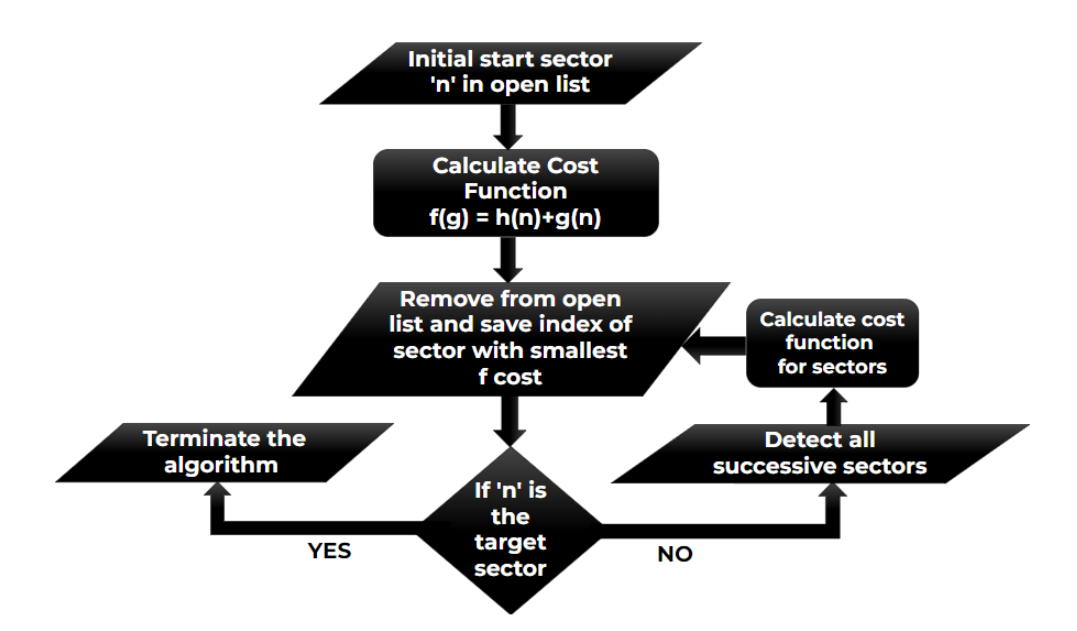
\includegraphics[width=1\textwidth]{Astar}
    \caption{Flowchart}
    \label{fig:pathPlanningFlowchart}
\end{figure}

\vspace{2cm}
\begin{algorithm}[hbt!]
    \caption{A* Path Planning}
    \label{alg:AStarAlgorithm}
    
    \begin{algorithmic}[1]
    
        \Require $ogrid \gets Occupancy \ grid \ data \ from \ RPLiDAR$
        \State $Define \ the \ start \ and \ end\ nodes$
        \State $First \ consider \ unoccupied \ neighbouring \ nodes \ of \ start \ node$
        \State $Evaluate \ G-cost \ and \ H-cost$
        \State $Add \ node \ with \ lowest \ F-cost \ to \ open \ set$
        \State $Consider \ neighboring \ nodes \ with \ lowest \ F-cost \ and \ repeat \ from \ step \ 3 $
        \State $Terminate \ the \ algorithm \ once \ H-cost \ is \ 0 $
        \State $Trace \ back \ last \ nodes\ to \ find \ optimum \ path$
        
    \end{algorithmic}
\end{algorithm}

For example, consider the graph shown below with nodes A, B, C and D interconnected with weighted edges, i.e., multiple distance values are associated with the graph.

\begin{figure}
    \centering
    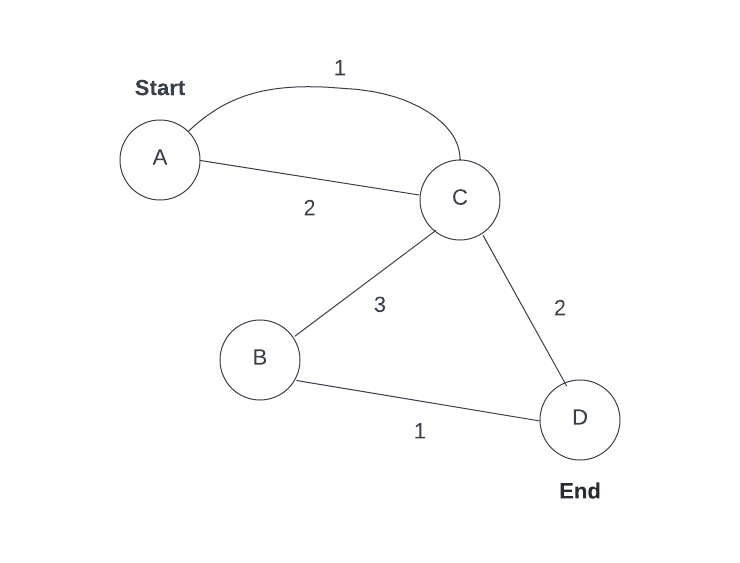
\includegraphics[width=0.45\textwidth]{nodesPath}
    \caption{Weighted graph with nodes A, B, C and D}
    \label{fig:weightedGraph}
\end{figure}

Here the Start node is A and the End node is D. The distance assciated with multiple paths are shown in figure. ie There are 2 ways from A to C, with distance values 1 and 2. The lowest weighted edge is chosen between these two. In this case, the shortest distance between them is 1 and that path is chosen. Thereafter reaching C the G-cost becomes 1 and so on. In the implementation these nodes are considered as the cells of the occupancy grid and the weights for the edges would be set to default as 1, because all the adjacent cells are in equal distances essentially. i.e. If the robot has to cross 2 cells to reach the destination, the distance or the cost would be 2. The intention of the algorithm would be to find the optimum path to reach the destination, here the optimum F-cost would 3 when the path A-C-D is traversed.

To start off with the algorithm we have to insert the start node, along with the F-cost ( initially 0), into the open set, represented by a priority queue. 

\[Open = \{(F-cost, \ Node)\} = \{(0, \ A)\}\]

The inital Costs of the respective nodes are represented in the table.Since we dont consider the start node as a neighbouring node all the values are set defuult to 0. while the other nodes B, C and D have a possibility of being considered as the Neighbouring node and thus the values are set as default to $\infty$. 

\begin{table}
\centering
    \begin{tabular}{ |c|c|c|c| } 
    \hline
    Nodes & F-cost & G-cost & H-cost \\
    \hline 
    A & 0 & 0 & 0\\ 
    B & $\infty$ & $\infty$ & $\infty$\\ 
    C & $\infty$ & $\infty$ & $\infty$\\ 
    D & $\infty$ & $\infty$ & $\infty$\\
    \hline
    \end{tabular}
    \caption{Nodes and their costs}
    \label{table:nodeCost0}
\end{table}

Now the first neighbouring node C is considered and the lowes G cost available to it is 1 and using the manhattan distance formula the h-cost is assumed to be 1 although the value might be incorrect. Then the overall f cost is 2. and the last node we came from is A. 

\begin{table}
\centering
    \begin{tabular}{ |c|c|c|c|c| } 
    \hline
    Nodes & F-cost & G-cost & H-cost & Last Node \\
    \hline 
    A & 0 & 0 & 0 &\\ 
    B & $\infty$ & $\infty$ & $\infty$ &\\ 
    C & 2 & 1 & 1 & A\\ 
    D & $\infty$ & $\infty$ & $\infty$ &\\
    \hline
    \end{tabular}
    \caption{Nodes and their costs}
    \label{table:nodeCost1}
\end{table}

Now this node aloong with its F-cost is added to the open set of neighbouring nodes.

\[Open = \{(2, \ C)\}\]

In the open set there is only one node so there is no comparisson to make with respect to the shortest F-cost.Now we consider the Node C and its neighbours, D and B. In the case of B the G-cost is 4 and H-cost is assumed, while in the case of D, the G-cost is 3. 
    The table is updated as shown below

\begin{table}
\centering
    \begin{tabular}{ |c|c|c|c|c| } 
    \hline
    Nodes & F-cost & G-cost & H-cost & Last Node \\
    \hline     
    A & 0 & 0 & 0 &\\ 
    B & 6 & 4 & 2 & C\\ 
    C & 2 & 1 & 1 & A\\ 
    D & 3 & 3 & 0 & C\\
    \hline
    \end{tabular}
    \caption{Nodes and their costs}
    \label{table:nodeCost2}
\end{table}

Therefore the node with the lower F-cost, D, is added to the open set and the node B is ignored.The value of H-cost is 0 for node D, since it is the end node.

\[Open = \{(2, \ C)\}, \{(3, \ D)\}\]

While comparing the F-costs of the nodes in the open set, we find the End node and its taken out of the open set to complete the algorithm.

Now all we have to do is backtrack all the last nodes. i.e. D from C, C from A, and thus we get the optimum path, A-C-D.

For the purpose of visualization additional python packages were used. \emph{PyGame} is a 2-D graphics module for python, which is easy to use and was used to implement the visualization tool effectively. 

The occupancy grid is generated from the data produced by the RPLiDAR unit. For purposes of visualization, we set the Start Node (in Orange), End node (in Turquoise), and Occupied Nodes (in Black), with the unoccupied Nodes represented in white. The reconstructed path is represented in purple, and is the optimum path for the robot to reach its destination.

The input and output images of the Pygame window are given in Figure \ref{fig:occupancyGrid} and Figure \ref{fig:reconstructedPath}.\\

\begin{figure}
    \begin{multicols}{2}
    \centering
        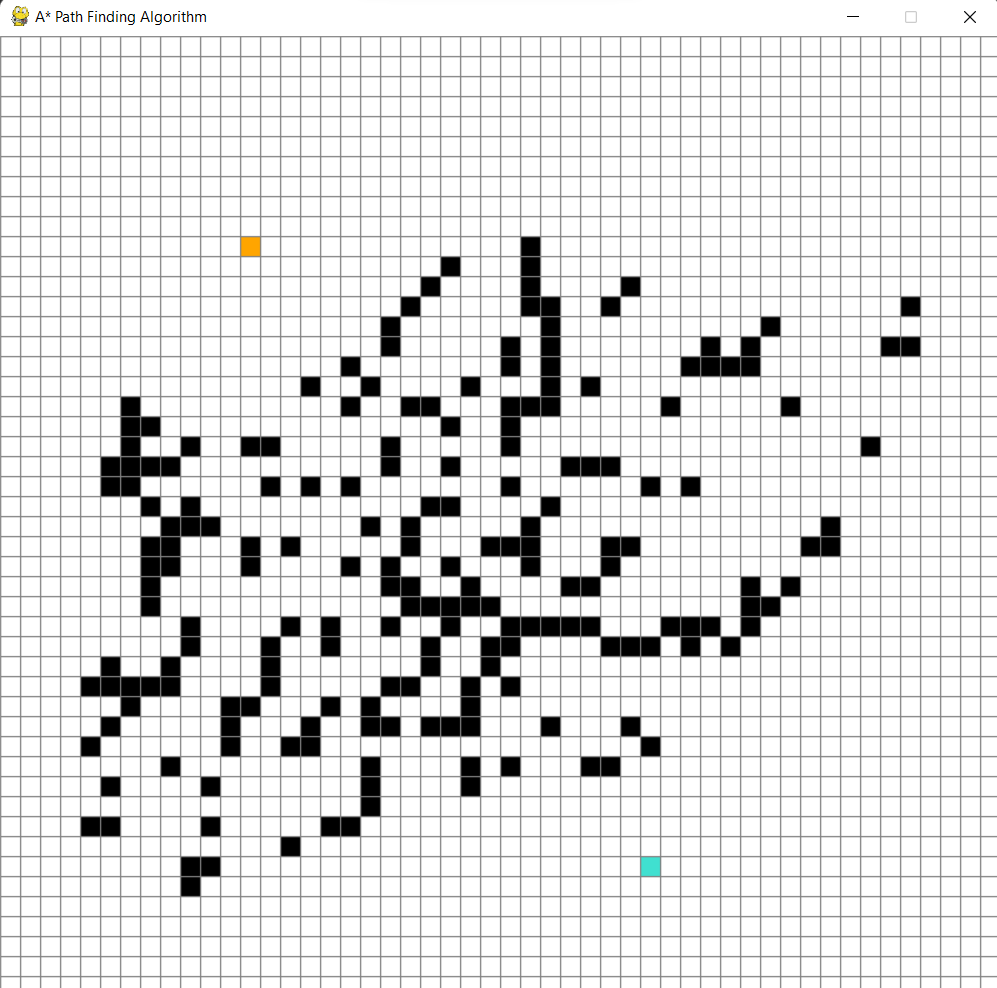
\includegraphics[width=0.35\textwidth]{Astarinput}\\
        \caption{Occupancy grid}
        \label{fig:occupancyGrid}

        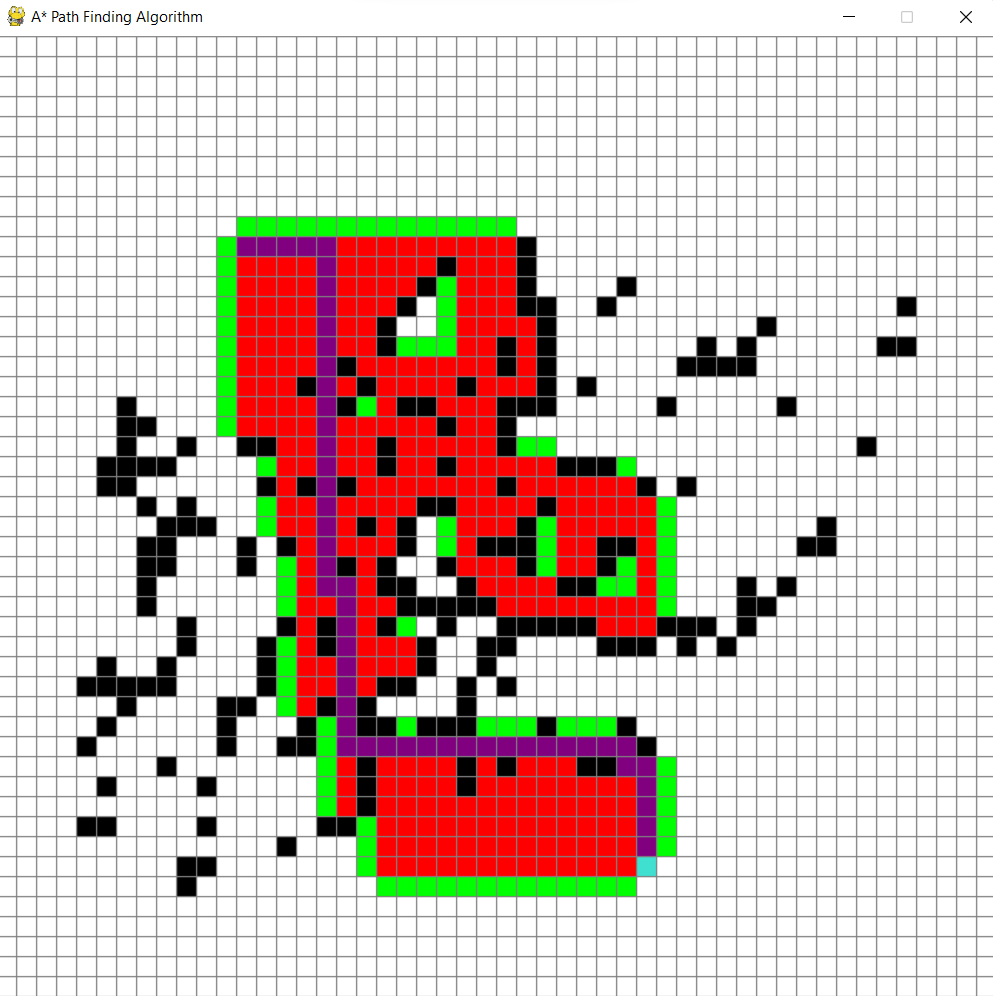
\includegraphics[width=0.35\textwidth]{Astaroutput}\\
        \caption{Reconstructed Path}
        \label{fig:reconstructedPath}
    \end{multicols}
\end{figure}





